\documentclass[a4paper]{article}
\usepackage[utf8]{inputenc}
\usepackage{amsmath}
\usepackage{graphicx}
\usepackage{indentfirst}
\usepackage{subfig}
\usepackage{float} % para usar [H]
%opening
\title{Tarea 2}
\author{María Victoria Jorge \\ 11-10495}

\begin{document}

\maketitle

\section{Clasificadores Lineales}
	En esta sección se presentarán los experimentos realizados para construir clasificadores lineales mediante aprendizaje con reforzamiento, un perceptrón de una capa y un adaline.\\
	
	Para la validación de todos los modelos se utilizará la técnica de validación cruzada. Además, se utilizará el porcentaje de datos bien clasificados como métrica de performance. Por último para asegurarnos que los modelos no están aprendiendo a clasificar basándose en el orden en que reciben los datos, en cada corrida los datos se desordenarán aleatoriamente.\\
	
	Como los datos presentados en el archivo lincloud3 tienen solo dos dimensiones, pueden graficarse e identificar fácilmente si
	son linealmente separables, para asegurarnos que los modelos utilizados a continuación serán capaces de clasificarlos. En la figura \ref{fig:datosOriginales} se tienen todos los datos identificados según la clase a la que pertenecen, y se puede observar que es posible trazar una línea entre ambas clases para separarlas.
	
	\begin{figure}[H]
	  \centering
	  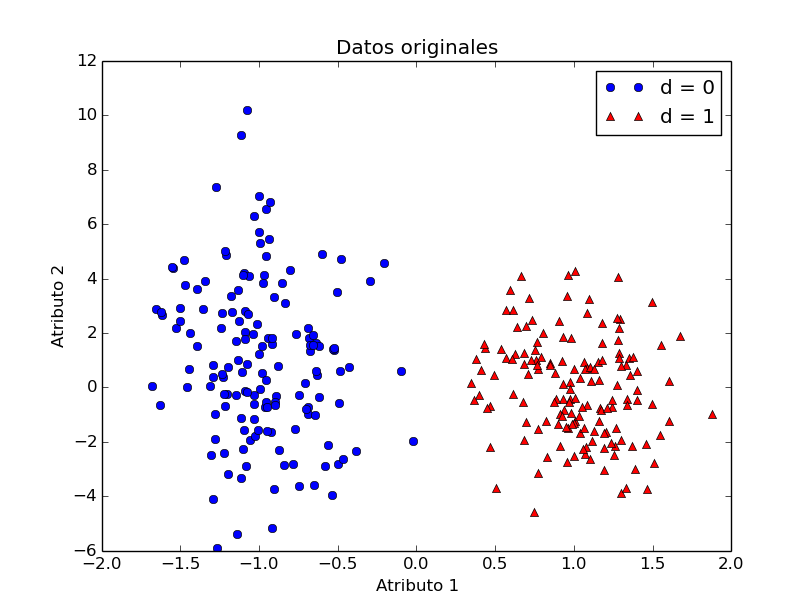
\includegraphics[scale=0.3]{datos.png}
	  \caption{Datos originales}
	  \label{fig:datosOriginales}
	\end{figure}
	
	\subsection{Aprendizaje con reforzamiento}
		Para estas pruebas se inicializaron los pesos de las dos neuronas en valores aleatorios entre -0.5 y 0.5, y se usaron esos mismos valores en todas las corridas. Como condición de parada para el entrenamiento se tomó que no existiera error en la clasificación de los datos o que se superara un número máximo de épocas (1000 épocas).
		
		En la Tabla \ref{tabla:accReforzamiento} se encuentran los resultados obtenidos de la ejecución de la validación cruzada 5-fold usando la red basada en aprendizaje con reforzamiento. 
		\begin{table}[H]
		\begin{center}
		\begin{tabular}{|l|l|l|l|l|}
		\hline
		Total datos & $\alpha$ & \% Correctos & \% Incorrectos & Épocas\\
		\hline \hline
		300 & 0.1 & 99.6667 & 0.3333 & 4.8 \\ \hline
		300 & 0.01 & 99.6667 & 0.3333 & 2\\ \hline
		300 & 0.001 & 99.3333 & 0.6667 & 4.2\\ \hline
		\end{tabular}
		\caption{Exactitud aprendizaje con reforzamiento}
		\label{tabla:accReforzamiento}
		\end{center}
		\end{table}
	
	\subsection{Perceptrón}
		Para estas pruebas se inicializaron los pesos en valores aleatorios entre -0.5 y 0.5, y se usaron esos mismos valores en todas las corridas. Se utilizó una sola neurona y la función de activación sgn o umbral. Como condición de parada para el entrenamiento se tomó que no existiera error en la clasificación de los datos o que se superara un número máximo de épocas (1000 épocas). Además se cambió la respuesta deseada de los datos cuyo valor era 0, por -1, para que coincidiera con el rango de valores que devuelve la función sgn.\\
		
		En la Tabla \ref{tabla:accPerceptron} se encuentran los resultados obtenidos luego de ejecutar validación cruzada con 5-fold para diferentes tasas de aprendizaje en una única neurona. Por cada iteración se utilizaron 240 datos para entrenar y 60 para probar el modelo. Luego de 5 iteraciones se probó en todos los experimentos con los 300 datos. El número de épocas indicado para cada tasa de aprendizaje es el promedio de los 5 entrenamientos realizados por tasa, con diferentes datos para entrenar en cada una.\\
		
		Con estos resultados puede observarse que al disminuir la tasa de aprendizaje el perceptrón necesita más épocas para cumplir con la cota de clasificar correctamente todos los datos de entrenamiento. Sin embargo, parece que al aumentar la cantidad de épocas para estos datos, el perceptrón tiene más problemas para clasificar los datos nuevos.
		
	
		\begin{table}[H]
		\begin{center}
		\begin{tabular}{|l|l|l|l|l|}
		\hline
		Total datos & $\alpha$ & \% Correctos & \% Incorrectos & Épocas\\
		\hline \hline
		300 & 0.1 & 99.6666 & 0.3334 & 3\\ \hline
		300 & 0.01 & 99.6666 & 0.3334 & 3.4\\ \hline
		300 & 0.001 & 99.3333 & 0.6667 & 15.2\\ \hline
		\end{tabular}
		\caption{Exactitud del perceptrón}
		\label{tabla:accPerceptron}
		\end{center}
		\end{table}
					
		Esto puede apreciarse de forma más clara con las gráficas de la figura \ref{f:perceptron}, donde se muestra para cada tasa de aprendizaje utilizada el peor hiperplano generado durante la validación cruzada. Podemos observar que en las tres figuras el hiperplano está muy cerca de las dos fronteras, lo que puede originar errores de clasificación cuando esos datos no se encuentran dentro del conjunto de entrenamiento, como sucedió en las gráficas \ref{f:perceptron2} y \ref{f:perceptron3}. Con esto se puede concluir que el modelo no está generalizando lo suficiente.			
				
		\begin{figure}[H]
		 \centering
		  \subfloat[$\alpha=0.1$]{
		   \label{f:perceptron1}
		    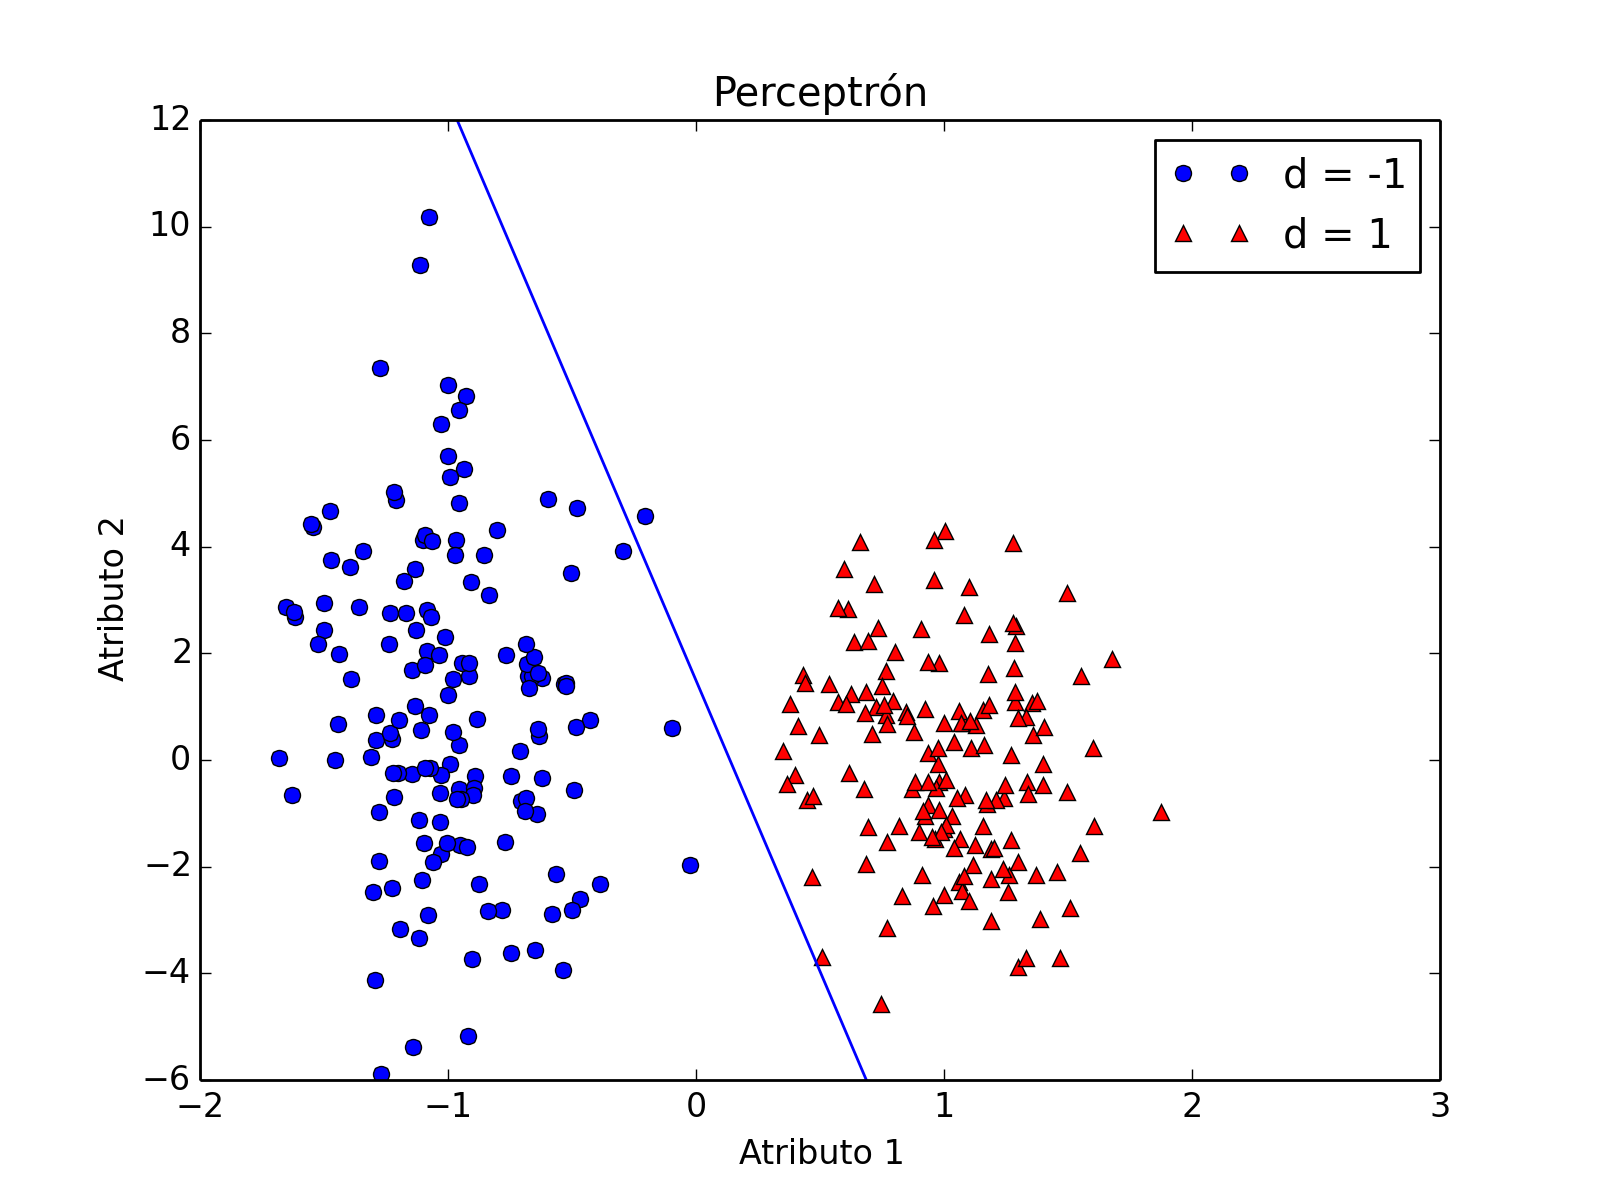
\includegraphics[width=0.3\textwidth]{perceptron.png}}
		  \subfloat[$\alpha=0.01$]{
		   \label{f:perceptron2}
		    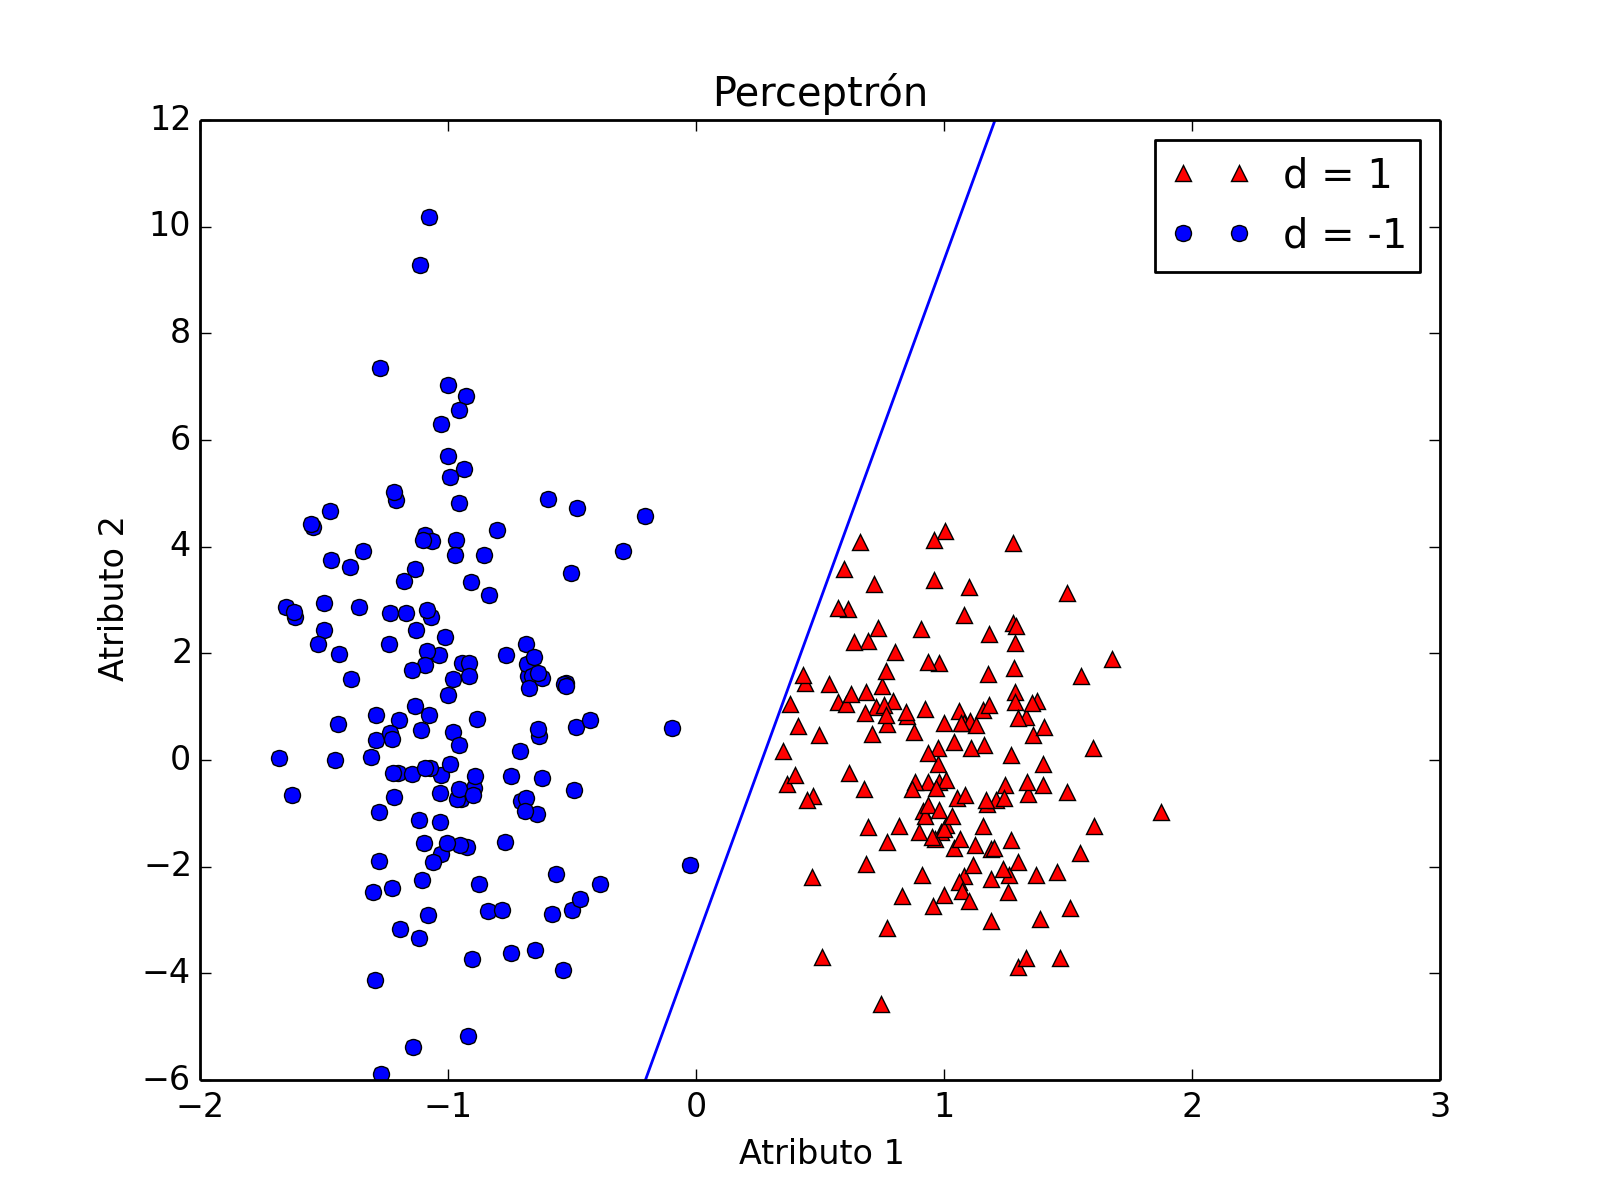
\includegraphics[width=0.3\textwidth]{perceptron_01.png}}
		  \subfloat[$\alpha=0.001$]{
		   \label{f:perceptron3}
		    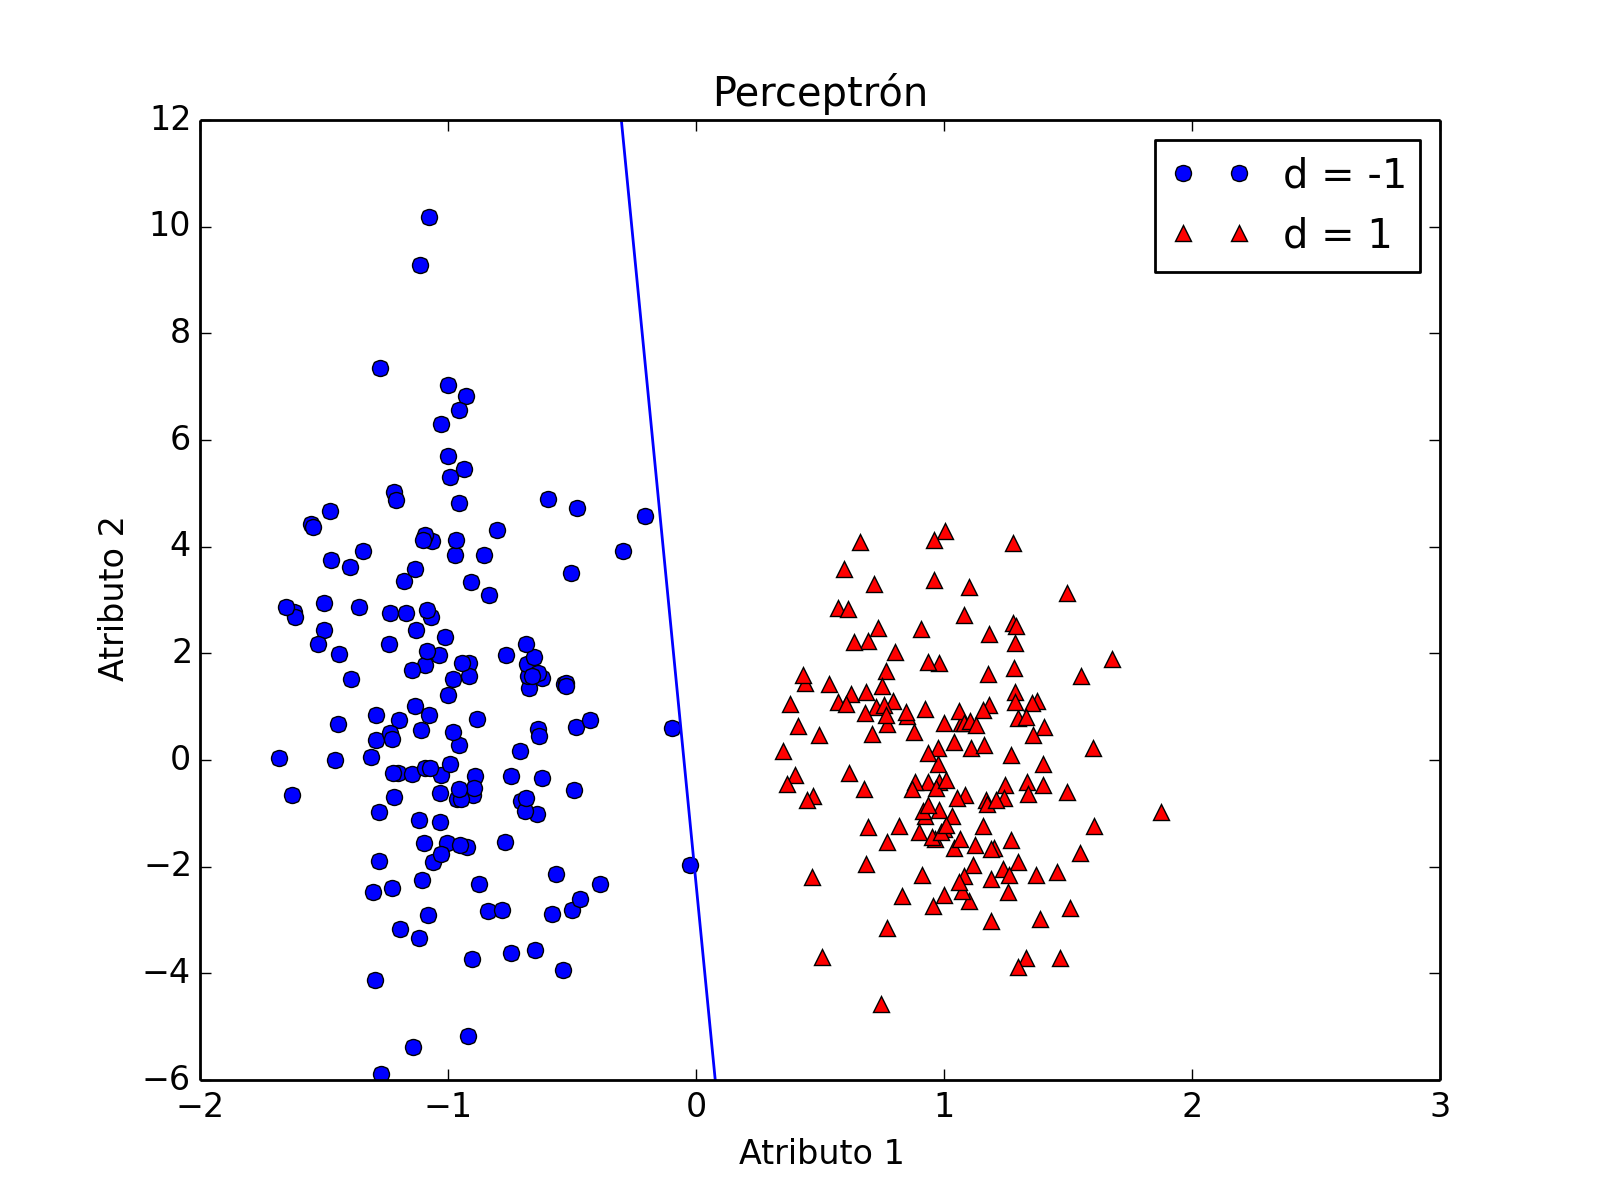
\includegraphics[width=0.3\textwidth]{perceptron_001.png}}
		 \caption{Modelos de perceptrón obtenidos en los tres experimentos}
		 \label{f:perceptron}
		\end{figure}
	
	\subsection{Adaline}
		Para estas pruebas se inicializaron los pesos de la neurona en valores aleatorios entre -0.5 y 0.5, manteniéndolos fijos durante todas las iteraciones de la validación cruzada de 5-fold. Como condición de parada para el algoritmo de entrenamiento se usó un máximo de 5000 épocas. Además, se modificó el archivo que contiene los datos para que las clases sean -1 y 1, en vez de 0 y 1 como estaban originalmente.\\
		
		En la Tabla \ref{tabla:accAdaline} se encuentran los resultados obtenidos para diferentes tasas de aprendizaje.
		Se puede observar que con tasas de aprendizaje muy pequeñas el Adaline converge mejor a la solución esperada, clasificando correctamente todos los datos.
		\begin{table}[H]
		\begin{center}
		\begin{tabular}{|l|l|l|l|l|}
		\hline
		Total datos & $\alpha$ & \% Correctos & \% Incorrectos & Épocas\\
		\hline \hline
		300 & 0.1 & 99.3333 & 0.6667 & 5000\\ \hline
		300 & 0.01 & 100 & 0 & 5000\\ \hline
		300 & 0.001 & 100 & 0 & 5000\\ \hline
		\end{tabular}
		\caption{Exactitud del Adaline}
		\label{tabla:accAdaline}
		\end{center}
		\end{table}
		
		Se realizaron pruebas con otras tasas de aprendizaje pero se presentaron las más significativas. El valor más alto con el que se obtuvieron buenos resultados fue $\alpha=0.1093$. Con valores más altos 5000 épocas no son suficientes para que el Adaline genere porcentajes tan altos de aciertos.
	
\section{Interpolador}
	El algoritmo de Adaline puede ser utilizado para iterpolación de funciones si se calcula la salida de la siguiente forma $y = a + b_{1}x + b_{2}x^{2} + ... + b_{k}x^{k}$ siendo k el grado del polinomio que se usará para interpolar. Siendo 'a' el sesgo, y cada $b_{i}$ los $w_{i}$ comunes del Adaline.\\
	
	Sabiendo esto debemos conocer cómo se comportan los datos que tenemos en p3data para saber el grado del polinomio con el que aproximaremos la función que los originó. Con la figura \ref{fig:interpolador} se puede apreciar que los datos parecen ser originados por una función cúbica, aunque tengan un poco de ruido.
	
	\begin{figure}[H]
	\centering
	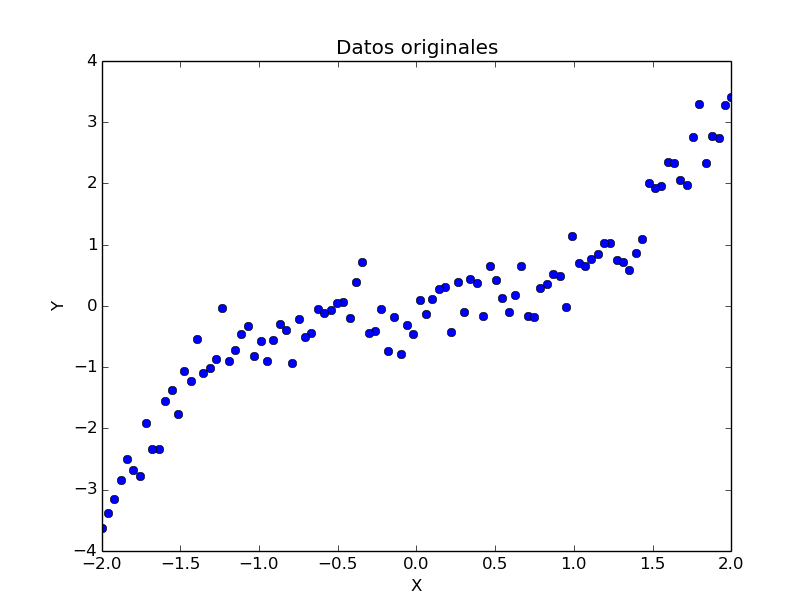
\includegraphics[scale=0.3]{interpolado.png}
	\caption{Datos originales a interpolar}
	\label{fig:interpolador}
	\end{figure}
	
	\begin{table}[H]
	\begin{center}
	\begin{tabular}{|l|l|l|l|l|}
	\hline
	Total datos & $\alpha$ & \% Correctos & \% Incorrectos & Épocas\\
	\hline \hline
	300 & 0.1 & 99.3333 & 0.6667 & 5000\\ \hline
	300 & 0.01 & 100 & 0 & 5000\\ \hline
	300 & 0.001 & 100 & 0 & 5000\\ \hline
	\end{tabular}
	\caption{Exactitud del Adaline como interpolador}
	\label{tabla:accInter}
	\end{center}
	\end{table}

\section{O-exclusivo}
Se demostrará que las clases del O-exclusivo (XOR) no son linealmente separables por reducción al absurdo.\\

Supongamos entonces que las clases del XOR son linealmente separables. Entonces existe un $\vec{w}^{t} = [w_{0}, w_{1}, w_{2}]^{t}$ que permite generar el hiperplano $\vec{w}^{t}\vec{x} = 0$ para un perceptrón de una neurona. Esta es la frontera que divide a las dos clases del XOR. Los datos que estén por debajo de esa frontera pertenecen a la clase 0, y los que están por encima pertenecen a la clase 1.\\

Por lo tanto se generan las siguientes ecuaciones:\\
\begin{equation}
0*w_{1} + 0*w_{2} + w_{0} <= 0 \iff w_{0} <= 0
\end{equation}
\begin{equation}
0*w_{1} + 1*w_{2} + w_{0} > 0 \iff w_{0} > -w_{2}
\end{equation}
\begin{equation}
1*w_{1} + 0*w_{2} + w_{0} > 0 \iff w_{0} > -w_{1}
\end{equation}
\begin{equation}
1*w_{1} + 1*w_{2} + w_{0} <= 0 \iff w_{0} <= -w_{1} - w_{2}
\end{equation}\\

De (1) obtenemos que $w_{0}$ es un número no positivo. Usando esta información en (2) y (3) tenemos que $w_{1}$ y $w_{2}$ son números positivos. \\

Luego, sabiendo que $w_{1}$ es positivo, podemos asegurar que $-w_{2} > -w_{2} -w_{1}$. Usando esta cota inferior en (2) se sigue cumpliendo que $w_{0} > -w_{2} - w_{1}$. Esto entra en contradicción con (4) que se obtuvo directamente del perceptrón. Por lo tanto la suposición que se hizo inicialmente sobre la separabilidad lineal de las clases del XOR es errónea.

\end{document}
